% Editable standalone vector figure extracted from novogaia_spectra.tex.
% Source slide 12; figure 12; native embedded fonts.
% Compile with LuaLaTeX from this directory, or run ../export_figures.py.
\documentclass[tikz,border=0pt]{standalone}
% Shared editable preamble for standalone, Nature-style vector figures.
% Text remains embedded and searchable. This is a house-style target, not a
% claim of acceptance or of satisfying every journal's submission checklist.
\usepackage{fontspec}
\setmainfont{LiberationSans}[
  Path=../assets/,Extension=.ttf,
  UprightFont=*-Regular,BoldFont=*-Bold,ItalicFont=*-Italic,BoldItalicFont=*-BoldItalic]
\setsansfont{LiberationSans}[
  Path=../assets/,Extension=.ttf,
  UprightFont=*-Regular,BoldFont=*-Bold,ItalicFont=*-Italic,BoldItalicFont=*-BoldItalic]
\setmonofont{LiberationSans}[
  Path=../assets/,Extension=.ttf,
  UprightFont=*-Regular,BoldFont=*-Bold,ItalicFont=*-Italic,BoldItalicFont=*-BoldItalic]
\usepackage{unicode-math}
\setmathfont{Latin Modern Math}
\DeclareMathSizes{5.9}{6}{5}{5}
\DeclareMathSizes{6}{6}{5}{5}
\usepackage{tikz}
\usetikzlibrary{arrows.meta,calc,positioning,patterns,decorations.pathreplacing,matrix}
\usepackage{graphicx}
\usepackage{xcolor}
\pagecolor{white}
\definecolor{ink}{HTML}{202020}
\definecolor{paper}{HTML}{FFFFFF}
\definecolor{muted}{HTML}{494949}
\definecolor{line}{HTML}{808080}
\definecolor{soft}{HTML}{F0F0F0}
\hyphenpenalty=10000\exhyphenpenalty=10000
\newcommand{\figurefont}{\sffamily\fontsize{5.9}{7.4}\selectfont}
\newcommand{\figuremathfont}{\sffamily\fontsize{6}{7.5}\selectfont}
\newcommand{\brandmedium}{\bfseries}
\renewcommand{\normalsize}{\figurefont}
\renewcommand{\small}{\figurefont}
\renewcommand{\footnotesize}{\figurefont}
\renewcommand{\scriptsize}{\figurefont}
\renewcommand{\tiny}{\figurefont}
\renewcommand{\large}{\figurefont}
\renewcommand{\Large}{\figurefont}
\renewcommand{\LARGE}{\figurefont}
\renewcommand{\huge}{\figurefont}
\renewcommand{\Huge}{\figurefont}
\tikzset{
  every path/.style={line width=.55pt},
  every node/.style={font=\figurefont,text=ink},
  arr/.style={-{Latex[length=1.5mm,width=1mm]},line width=.55pt,draw=ink},
  thinarr/.style={-{Latex[length=1.3mm,width=.9mm]},line width=.55pt,draw=ink},
  box/.style={draw=ink,line width=.55pt,fill=white,minimum height=.85cm,align=center,inner sep=3pt},
  ghost/.style={draw=muted,dashed,fill=soft},
  tag/.style={font=\figurefont,text=muted},
  equ/.style={font=\figuremathfont},
  small/.style={font=\figurefont},
  body/.style={font=\figurefont},
  tinytext/.style={font=\figurefont}
}
\newcommand{\txt}[4]{\node[anchor=north west,align=left,text width=#3cm] at (#1,#2) {#4};}
\newcommand{\smalltxt}[4]{\node[anchor=north west,align=left,text width=#3cm,small] at (#1,#2) {#4};}
\newcommand{\eqn}[4][6]{\node[anchor=north west,font=\figuremathfont] at (#2,#3) {$\displaystyle #4$};}
\newcommand{\diagramblock}[5]{\node[box,minimum width=#3cm,text width=#3cm,minimum height=#4cm] at (#1,#2) {#5};}
% Scale coordinates, not text: all labels retain one final publication size.
\newcommand{\spectrum}[3]{\begin{scope}[shift={(#1,#2)}]
  \draw[muted] (0,0)--({3.6*#3},0);
  \draw[muted] (0,0)--(0,{1.9*#3});
  \foreach \x/\h in {.25/.18,.49/.46,.68/1.42,.87/.37,1.08/.74,1.31/.31,1.57/1.78,1.76/.46,1.96/.19,2.17/1.1,2.37/.57,2.57/.31,2.88/.76,3.21/.23,3.4/.38}{
    \draw[ink] ({\x*#3},0)--({\x*#3},{\h*#3});}
  \foreach \x in {.6,1.2,1.8,2.4,3.0}{\draw[ink] ({\x*#3},0)--+(0,{-.06*#3});}
  \foreach \y in {.45,.9,1.35,1.8}{\draw[ink] (0,{\y*#3})--+({-.06*#3},0);}
  \foreach \x/\lab in {0/0,1.8/45,3.6/90}{\node[anchor=north,font=\figurefont] at ({\x*#3},{-.08*#3}) {\lab};}
  \foreach \y/\lab in {0/0,.9/0.5,1.8/1.0}{\node[anchor=east,font=\figurefont] at ({-.08*#3},{\y*#3}) {\lab};}
  \node[anchor=north east,font=\figurefont] at ({3.6*#3},{-.45*#3}) {$m/z$ (Th)};
  \node[anchor=south west,font=\figurefont] at (0,{1.96*#3}) {Relative intensity (a.u.)};
\end{scope}}
\newcommand{\molecule}[3]{\begin{scope}[shift={(#1,#2)}]
  \draw[ink] (0,{#3})--({.866*#3},{.5*#3})--({.866*#3},{-.5*#3})--(0,{-#3})--({-.866*#3},{-.5*#3})--({-.866*#3},{.5*#3})--cycle;
  \draw[ink] ({.68*#3},{.4*#3})--({.68*#3},{-.4*#3});
  \draw[ink] ({-.7*#3},{-.44*#3})--({-.02*#3},{-.83*#3});
  \draw[ink] ({-.7*#3},{.44*#3})--({-.02*#3},{.83*#3});
  \draw[ink] (0,{#3})--(0,{1.55*#3});
  \node[font=\figurefont] at (0,{1.77*#3}) {OH};
\end{scope}}
\newcommand{\peaktokens}[3]{\foreach \i in {0,...,5}{\pgfmathsetmacro{\xx}{#1+\i*.36}\draw[fill=#3,draw=ink] (\xx,#2) rectangle +(.24,.6);}}
\newcommand{\E}{\mathbb E}
\newcommand{\R}{\mathbb R}
\newcommand{\sg}{\operatorname{stopgrad}}
\newcommand{\LN}{\operatorname{LN}}
\newcommand{\softmax}{\operatorname{softmax}}

\begin{document}
\figurefont
\begin{tikzpicture}[x=1cm,y=1cm,scale=1.14375,transform shape]
% A fixed teacher defines the same scalar target for this one input.
\node[small,anchor=base,inner sep=0] at (2.5,6.64) {Same spectrum $S$};
\draw[muted,line width=.55pt] (1.42,5.80)--(3.55,5.80);
\draw[muted,line width=.55pt] (1.42,5.80)--(1.42,6.48);
\foreach \x/\h in {.16/.16,.36/.48,.58/.25,.82/.60,1.06/.19,1.27/.40,1.52/.22,1.81/.30,1.98/.16}{\draw[ink,line width=.55pt] (1.42+\x,5.80)--+(0,\h);}
\node[tinytext,anchor=north,inner sep=1pt] at (2.49,5.73) {$m/z$ (Th; schematic)};
\node[tinytext,rotate=90,inner sep=0] at (1.14,6.14) {$I/I_{\max}$};
\node[box,minimum width=2.45cm,minimum height=.66cm,inner sep=4pt] (teacher) at (7.68,6.15) {Frozen teacher $T$};
\draw[arr] (3.85,6.15)--(teacher.west);
\node[small,anchor=base,inner sep=0] at (12.18,6.67) {Fixed target $Y$};
\draw[ink,fill=soft,line width=.55pt] (11.73,5.80) rectangle (12.63,6.50);
\node[font=\figurefont,inner sep=0] at (12.18,6.15) {$4$};
\draw[arr] (teacher.east)--(11.58,6.15);
% Two equally valid student/predictor factorizations, not a training sequence.
\node[small,anchor=base,inner sep=0] at (2.77,5.01) {Student code $Z$};
\node[small,anchor=base,inner sep=0] at (7.68,5.01) {Predictor $g$};
\node[small,anchor=base,inner sep=0] at (12.18,5.01) {Prediction $\widehat Y$};
\foreach \y/\name/\code/\operation in {4.34/A/2/{\times 2},3.11/B/8/{\div 2}}{
 \node[small,anchor=west,inner sep=0] at (1.05,\y) {Code \name};
 \draw[ink,fill=soft,line width=.55pt] (2.63,\y-.35) rectangle (3.53,\y+.35);
 \node[font=\figurefont,inner sep=0] at (3.08,\y) {$\code$};
 \node[box,minimum width=2.45cm,minimum height=.70cm,inner sep=4pt] (pred\name) at (7.68,\y) {$\operation$};
 \draw[arr] (3.68,\y)--(pred\name.west);
 \draw[ink,fill=soft,line width=.55pt] (11.73,\y-.35) rectangle (12.63,\y+.35);
 \node[font=\figurefont,inner sep=0] at (12.18,\y) {$4$};
 \draw[arr] (pred\name.east)--(11.58,\y);}
\draw[muted,dashed,line width=.55pt] (12.80,6.15)--(13.45,6.15)--(13.45,3.11)--(12.80,3.11);
\draw[muted,dashed,line width=.55pt] (12.80,4.34)--(13.45,4.34);
\node[small,anchor=west,inner sep=0,align=left] at (13.73,4.69) {Both\\match};
\node[anchor=base,inner sep=0,font=\figurefont] at (8.02,2.23) {$\widehat Y=g(Z),\qquad\mathcal L=\tfrac12(\widehat Y-Y)^2$};
% Fixed canvas: 183 x 60.046875 mm. No clipping: overflow is audited.
\pgfresetboundingbox
\path[use as bounding box] (0,1.6) rectangle (16,6.85);
\end{tikzpicture}
\end{document}
